% Options for packages loaded elsewhere
\PassOptionsToPackage{unicode}{hyperref}
\PassOptionsToPackage{hyphens}{url}
\PassOptionsToPackage{dvipsnames,svgnames,x11names}{xcolor}
%
\documentclass[
  letterpaper,
  DIV=11,
  numbers=noendperiod]{scrartcl}

\usepackage{amsmath,amssymb}
\usepackage{lmodern}
\usepackage{iftex}
\ifPDFTeX
  \usepackage[T1]{fontenc}
  \usepackage[utf8]{inputenc}
  \usepackage{textcomp} % provide euro and other symbols
\else % if luatex or xetex
  \usepackage{unicode-math}
  \defaultfontfeatures{Scale=MatchLowercase}
  \defaultfontfeatures[\rmfamily]{Ligatures=TeX,Scale=1}
\fi
% Use upquote if available, for straight quotes in verbatim environments
\IfFileExists{upquote.sty}{\usepackage{upquote}}{}
\IfFileExists{microtype.sty}{% use microtype if available
  \usepackage[]{microtype}
  \UseMicrotypeSet[protrusion]{basicmath} % disable protrusion for tt fonts
}{}
\makeatletter
\@ifundefined{KOMAClassName}{% if non-KOMA class
  \IfFileExists{parskip.sty}{%
    \usepackage{parskip}
  }{% else
    \setlength{\parindent}{0pt}
    \setlength{\parskip}{6pt plus 2pt minus 1pt}}
}{% if KOMA class
  \KOMAoptions{parskip=half}}
\makeatother
\usepackage{xcolor}
\setlength{\emergencystretch}{3em} % prevent overfull lines
\setcounter{secnumdepth}{-\maxdimen} % remove section numbering
% Make \paragraph and \subparagraph free-standing
\ifx\paragraph\undefined\else
  \let\oldparagraph\paragraph
  \renewcommand{\paragraph}[1]{\oldparagraph{#1}\mbox{}}
\fi
\ifx\subparagraph\undefined\else
  \let\oldsubparagraph\subparagraph
  \renewcommand{\subparagraph}[1]{\oldsubparagraph{#1}\mbox{}}
\fi

\usepackage{color}
\usepackage{fancyvrb}
\newcommand{\VerbBar}{|}
\newcommand{\VERB}{\Verb[commandchars=\\\{\}]}
\DefineVerbatimEnvironment{Highlighting}{Verbatim}{commandchars=\\\{\}}
% Add ',fontsize=\small' for more characters per line
\usepackage{framed}
\definecolor{shadecolor}{RGB}{241,243,245}
\newenvironment{Shaded}{\begin{snugshade}}{\end{snugshade}}
\newcommand{\AlertTok}[1]{\textcolor[rgb]{0.68,0.00,0.00}{#1}}
\newcommand{\AnnotationTok}[1]{\textcolor[rgb]{0.37,0.37,0.37}{#1}}
\newcommand{\AttributeTok}[1]{\textcolor[rgb]{0.40,0.45,0.13}{#1}}
\newcommand{\BaseNTok}[1]{\textcolor[rgb]{0.68,0.00,0.00}{#1}}
\newcommand{\BuiltInTok}[1]{\textcolor[rgb]{0.00,0.23,0.31}{#1}}
\newcommand{\CharTok}[1]{\textcolor[rgb]{0.13,0.47,0.30}{#1}}
\newcommand{\CommentTok}[1]{\textcolor[rgb]{0.37,0.37,0.37}{#1}}
\newcommand{\CommentVarTok}[1]{\textcolor[rgb]{0.37,0.37,0.37}{\textit{#1}}}
\newcommand{\ConstantTok}[1]{\textcolor[rgb]{0.56,0.35,0.01}{#1}}
\newcommand{\ControlFlowTok}[1]{\textcolor[rgb]{0.00,0.23,0.31}{#1}}
\newcommand{\DataTypeTok}[1]{\textcolor[rgb]{0.68,0.00,0.00}{#1}}
\newcommand{\DecValTok}[1]{\textcolor[rgb]{0.68,0.00,0.00}{#1}}
\newcommand{\DocumentationTok}[1]{\textcolor[rgb]{0.37,0.37,0.37}{\textit{#1}}}
\newcommand{\ErrorTok}[1]{\textcolor[rgb]{0.68,0.00,0.00}{#1}}
\newcommand{\ExtensionTok}[1]{\textcolor[rgb]{0.00,0.23,0.31}{#1}}
\newcommand{\FloatTok}[1]{\textcolor[rgb]{0.68,0.00,0.00}{#1}}
\newcommand{\FunctionTok}[1]{\textcolor[rgb]{0.28,0.35,0.67}{#1}}
\newcommand{\ImportTok}[1]{\textcolor[rgb]{0.00,0.46,0.62}{#1}}
\newcommand{\InformationTok}[1]{\textcolor[rgb]{0.37,0.37,0.37}{#1}}
\newcommand{\KeywordTok}[1]{\textcolor[rgb]{0.00,0.23,0.31}{#1}}
\newcommand{\NormalTok}[1]{\textcolor[rgb]{0.00,0.23,0.31}{#1}}
\newcommand{\OperatorTok}[1]{\textcolor[rgb]{0.37,0.37,0.37}{#1}}
\newcommand{\OtherTok}[1]{\textcolor[rgb]{0.00,0.23,0.31}{#1}}
\newcommand{\PreprocessorTok}[1]{\textcolor[rgb]{0.68,0.00,0.00}{#1}}
\newcommand{\RegionMarkerTok}[1]{\textcolor[rgb]{0.00,0.23,0.31}{#1}}
\newcommand{\SpecialCharTok}[1]{\textcolor[rgb]{0.37,0.37,0.37}{#1}}
\newcommand{\SpecialStringTok}[1]{\textcolor[rgb]{0.13,0.47,0.30}{#1}}
\newcommand{\StringTok}[1]{\textcolor[rgb]{0.13,0.47,0.30}{#1}}
\newcommand{\VariableTok}[1]{\textcolor[rgb]{0.07,0.07,0.07}{#1}}
\newcommand{\VerbatimStringTok}[1]{\textcolor[rgb]{0.13,0.47,0.30}{#1}}
\newcommand{\WarningTok}[1]{\textcolor[rgb]{0.37,0.37,0.37}{\textit{#1}}}

\providecommand{\tightlist}{%
  \setlength{\itemsep}{0pt}\setlength{\parskip}{0pt}}\usepackage{longtable,booktabs,array}
\usepackage{calc} % for calculating minipage widths
% Correct order of tables after \paragraph or \subparagraph
\usepackage{etoolbox}
\makeatletter
\patchcmd\longtable{\par}{\if@noskipsec\mbox{}\fi\par}{}{}
\makeatother
% Allow footnotes in longtable head/foot
\IfFileExists{footnotehyper.sty}{\usepackage{footnotehyper}}{\usepackage{footnote}}
\makesavenoteenv{longtable}
\usepackage{graphicx}
\makeatletter
\def\maxwidth{\ifdim\Gin@nat@width>\linewidth\linewidth\else\Gin@nat@width\fi}
\def\maxheight{\ifdim\Gin@nat@height>\textheight\textheight\else\Gin@nat@height\fi}
\makeatother
% Scale images if necessary, so that they will not overflow the page
% margins by default, and it is still possible to overwrite the defaults
% using explicit options in \includegraphics[width, height, ...]{}
\setkeys{Gin}{width=\maxwidth,height=\maxheight,keepaspectratio}
% Set default figure placement to htbp
\makeatletter
\def\fps@figure{htbp}
\makeatother

\usepackage{booktabs}
\usepackage{longtable}
\usepackage{array}
\usepackage{multirow}
\usepackage{wrapfig}
\usepackage{float}
\usepackage{colortbl}
\usepackage{pdflscape}
\usepackage{tabu}
\usepackage{threeparttable}
\usepackage{threeparttablex}
\usepackage[normalem]{ulem}
\usepackage{makecell}
\usepackage{xcolor}
\usepackage{float}
\usepackage{bm}
\usepackage{cancel}
\usepackage{dsfont}
\usepackage{framed}
\usepackage{mathtools}
\usepackage{soul}
\usepackage{amsmath,amssymb,latexsym}
\addtokomafont{disposition}{\rmfamily}
\DeclareMathOperator*{\argmax}{arg\,max}
\DeclareMathOperator*{\argmin}{arg\,min}
\newcommand{\items}[1]{\begin{itemize} #1 \end{itemize}}
\newcommand{\enums}[1]{\begin{enumerate} #1 \end{enumerate}}
\newcommand{\E}{\mathbb{E}}
\newcommand{\V}{\mathbb{V}}
\newcommand{\Cov}{\text{Cov}}
\newcommand{\R}{\mathbb{R}}
\newcommand{\T}{\mathtt{T}}
\renewcommand{\P}{\mathbb{P}}
\newcommand{\supp}[1]{\text{supp}(#1)}
\newcommand\independent{\perp\!\!\!\perp}
\def\independenT#1#2{\mathrel{\rlap{$#1#2$}\mkern2mu{#1#2}}}
\newcommand*{\vertbar}{\rule[-1ex]{0.5pt}{2.5ex}}
\newcommand*{\horzbar}{\rule[.5ex]{2.5ex}{0.5pt}}
% \renewcommand{\d}[0]{\mathrm{d}}
\newcommand{\pp}[2][]{\frac{\partial#1}{\partial#2}}
\newcommand{\dd}[2][]{\frac{\mathrm d#1}{\mathrm d#2}}
\KOMAoption{captions}{tableheading}
\makeatletter
\@ifpackageloaded{tcolorbox}{}{\usepackage[many]{tcolorbox}}
\@ifpackageloaded{fontawesome5}{}{\usepackage{fontawesome5}}
\definecolor{quarto-callout-color}{HTML}{909090}
\definecolor{quarto-callout-note-color}{HTML}{0758E5}
\definecolor{quarto-callout-important-color}{HTML}{CC1914}
\definecolor{quarto-callout-warning-color}{HTML}{EB9113}
\definecolor{quarto-callout-tip-color}{HTML}{00A047}
\definecolor{quarto-callout-caution-color}{HTML}{FC5300}
\definecolor{quarto-callout-color-frame}{HTML}{acacac}
\definecolor{quarto-callout-note-color-frame}{HTML}{4582ec}
\definecolor{quarto-callout-important-color-frame}{HTML}{d9534f}
\definecolor{quarto-callout-warning-color-frame}{HTML}{f0ad4e}
\definecolor{quarto-callout-tip-color-frame}{HTML}{02b875}
\definecolor{quarto-callout-caution-color-frame}{HTML}{fd7e14}
\makeatother
\makeatletter
\makeatother
\makeatletter
\makeatother
\makeatletter
\@ifpackageloaded{caption}{}{\usepackage{caption}}
\AtBeginDocument{%
\ifdefined\contentsname
  \renewcommand*\contentsname{Table of contents}
\else
  \newcommand\contentsname{Table of contents}
\fi
\ifdefined\listfigurename
  \renewcommand*\listfigurename{List of Figures}
\else
  \newcommand\listfigurename{List of Figures}
\fi
\ifdefined\listtablename
  \renewcommand*\listtablename{List of Tables}
\else
  \newcommand\listtablename{List of Tables}
\fi
\ifdefined\figurename
  \renewcommand*\figurename{Figure}
\else
  \newcommand\figurename{Figure}
\fi
\ifdefined\tablename
  \renewcommand*\tablename{Table}
\else
  \newcommand\tablename{Table}
\fi
}
\@ifpackageloaded{float}{}{\usepackage{float}}
\floatstyle{ruled}
\@ifundefined{c@chapter}{\newfloat{codelisting}{h}{lop}}{\newfloat{codelisting}{h}{lop}[chapter]}
\floatname{codelisting}{Listing}
\newcommand*\listoflistings{\listof{codelisting}{List of Listings}}
\makeatother
\makeatletter
\@ifpackageloaded{caption}{}{\usepackage{caption}}
\@ifpackageloaded{subcaption}{}{\usepackage{subcaption}}
\makeatother
\makeatletter
\@ifpackageloaded{tcolorbox}{}{\usepackage[many]{tcolorbox}}
\makeatother
\makeatletter
\@ifundefined{shadecolor}{\definecolor{shadecolor}{rgb}{.97, .97, .97}}
\makeatother
\makeatletter
\makeatother
\ifLuaTeX
  \usepackage{selnolig}  % disable illegal ligatures
\fi
\IfFileExists{bookmark.sty}{\usepackage{bookmark}}{\usepackage{hyperref}}
\IfFileExists{xurl.sty}{\usepackage{xurl}}{} % add URL line breaks if available
\urlstyle{same} % disable monospaced font for URLs
\hypersetup{
  pdftitle={Homework 1 --- BST 258: Causal Inference, Theory and Practice},
  pdfauthor={Christian Testa},
  colorlinks=true,
  linkcolor={blue},
  filecolor={Maroon},
  citecolor={Blue},
  urlcolor={Blue},
  pdfcreator={LaTeX via pandoc}}

\title{Homework 1 --- BST 258: Causal Inference, Theory and Practice}
\usepackage{etoolbox}
\makeatletter
\providecommand{\subtitle}[1]{% add subtitle to \maketitle
  \apptocmd{\@title}{\par {\large #1 \par}}{}{}
}
\makeatother
\subtitle{Due February 16th, 2024, 5:00 PM}
\author{Christian Testa}
\date{}

\begin{document}
\maketitle
\ifdefined\Shaded\renewenvironment{Shaded}{\begin{tcolorbox}[sharp corners, breakable, borderline west={3pt}{0pt}{shadecolor}, boxrule=0pt, interior hidden, enhanced, frame hidden]}{\end{tcolorbox}}\fi

\hypertarget{question-1}{%
\subsection{Question 1}\label{question-1}}

Done \(\checkmark\)

Find my homework repository at
\url{https://github.com/ctesta01/bst258_hw1/}

\hypertarget{question-2}{%
\subsection{Question 2}\label{question-2}}

Consider a completely randomized experiment (CRE) with
\(i = 1, \ldots, n\) units, \(m\) of which are treated, where \(A_i\) is
1 when unit \(i\) is treated.

\begin{enumerate}
\def\labelenumi{\alph{enumi})}
\item
  What is the marginal distribution of the treatment indicator \(A\)?
\item
  What is the joint distribution of \(A_i\) and \(A_j\) for two units
  \(i \neq j\)? (Hint: This amounts to completing a contingency table.)
\item
  What are \(\V(A_i)\) and \(\text{Cov}(A_i, A_j)\) for \(i \neq j\)?
\item
  The \emph{sample} Average Treatment Effect on the Treated (ATT) is
  \(\theta^{ATT} = \frac{1}{m} \sum_{i=1}^{n} A_i(Y_i(1) - Y_i(0))\).
  What is the sample ATT in expectation?
\end{enumerate}

\hypertarget{answer-to-question-2}{%
\subsection{Answer to Question 2}\label{answer-to-question-2}}

\begin{enumerate}
\def\labelenumi{\alph{enumi})}
\tightlist
\item
  The marginal distribution is \(P(A = 1) = m/n\).
\item
  The joint distribution is given by the following probabilities, where
  \(i \neq j\):
\end{enumerate}

\begin{itemize}
\tightlist
\item
  \(\P(A_i = A_j = 1) = \left( \frac{m}{n} \right) \left( \frac{m-1}{n-1} \right)\),
\item
  \(\P(A_i = 1, A_j = 0) = \left( \frac{m}{n} \right) \left( \frac{n-m-1}{n-1} \right)\),
\item
  \(\P(A_j = 0, A_j = 1) = \left( \frac{m}{n} \right) \left( \frac{n-m-1}{n-1} \right)\),
\item
  \(\P(A_j = A_j = 0) = \left( \frac{n-m}{n} \right) \left( \frac{n-m-1}{n-1} \right)\).
\end{itemize}

\begin{enumerate}
\def\labelenumi{\alph{enumi})}
\setcounter{enumi}{2}
\tightlist
\item
  Let \(p = m/n\). Then
  \(\V[A_i] = \E[A_i^2] - \E[A_i]^2 = p - p^2 = p(1-p)\).
  \(\Cov(A_i, A_j) = \E[(A_i - \E[A_i])(A_j - \E[A_j])] = (p - p)(p-p) = 0\),
  where we used that \(A_i \independent A_j\) to break apart the
  expectation.
\item
  The expectation of the average treatment effect on the treated is
  given by \[
    \begin{aligned}
    \E[\theta^{\text{ATT}}] & = \E[\frac{1}{m} \sum_{i=1}^n A_i (Y_i(1) - Y_i(0))] \\
    & = \frac{1}{m} \sum_{i=1}^n \E[A_i Y_i(1)] - \frac{1}{m} \sum_{i=1}^n \E[A_i Y_i(0)] \\ 
    & = \frac{1}{m} \sum_{i=1}^n p \E[Y_i(1)] - \frac{1}{m} \sum_{i=1}^n p \E[Y_i(0)] \\ 
    & = \frac{1}{n} n (\E[Y_i(1)] - \E[Y_i(0)]) \\ 
    & = \E[Y_i(1) - Y_i(0)] \\ 
    & = \theta^{\text{ATE}}.
    \end{aligned}
    \]
\end{enumerate}

\newpage

\hypertarget{question-3}{%
\subsection{Question 3}\label{question-3}}

Consider an additive treatment effect model, i.e.,
\(\theta = Y_i(1) - Y_i(0)\) for all \(i\), so
\(Y_i(1) = Y_i(0) + \theta\). Show that \(\V(Y_i(1)) = \V(Y_i(0))\) and
that the correlation \(\rho(Y_i(1), Y_i(0)) = 1\), where expectations
are sample expectations, i.e.,
\(\E[Y_i(1)] = \frac{1}{n} \sum_{i=1}^{n} Y_i(1)\).

\hypertarget{answer-to-question-3}{%
\subsection{Answer to Question 3}\label{answer-to-question-3}}

If \(Y_i(1) = Y_i(0) + \theta\), then
\(\V(Y_i(1)) = \V(Y_i(0) + \theta) = \V(Y_i(0))\). This also implies
that \(\sigma_{Y_i(1)} = \sigma_{Y_i(0)}\).

The sample correlation will be given by \[
\rho(Y_i(1), Y_i(0)) = 
\frac{\text{Cov}(Y_i(1), Y_i(0))}{\sigma_{Y_i(1)} \sigma_{Y_i(0)}} = \\ 
\frac{\E(Y_i(1) - \E[Y_i(1)])(Y_i(1) - \cancel{\theta} - \E[Y_i(1)] + \cancel{\theta})}{\V(Y_i(1))} = 
\frac{\V(Y_i(1))}{\V(Y_i(1))} = 1.
\]

\newpage

\hypertarget{question-4}{%
\subsection{Question 4}\label{question-4}}

It's tea time: (a hologram of) R.A. Fisher places eight cups of tea
(with milk) in front of you and asks you to identify which cups had tea
poured before milk and vice-versa. Prior to giving you the cups of tea,
Fisher poured milk before tea in four of them and tea before milk in the
other four. The ordering in which the cups have been served is random.
What is the probability that you correctly guess 0, 1, 2, 3, or 4 of all
of the cups that had tea poured first?

\hypertarget{answer-to-question-4}{%
\subsection{Answer to Question 4}\label{answer-to-question-4}}

This scenario can be modelled as a hypergeometrically distributed random
variable \(K\) representing the number of correct guesses.

Let \(\mathbb M\) be the set of cups where milk was poured first, and
\(\mathbb T\) be the set of cups where tea was poured first, such that
\(|\mathbb M| = |\mathbb T| = 4\).

We are guessing 4 cups for which we speculate milk was poured first. As
such, the probability that we guess \(K = k\) correctly is given by

\[\P(K = k) = \frac{{\mathbb M \choose k} {\mathbb T \choose 4-k}}{{\mathbb M + \mathbb T \choose 4}}.
\]

The exact probabilities are given in the following table:

\begin{longtable}[]{@{}lll@{}}
\toprule()
\(K = k\) & \(\P(K = k)\) & \(\P(K = k)\) in decimal \\
\midrule()
\endhead
0 & 1/70 & 0.014 \\
1 & 16/70 & 0.229 \\
2 & 36/70 & 0.514 \\
3 & 16/70 & 0.229 \\
4 & 1/70 & 0.014 \\
\bottomrule()
\end{longtable}

\newpage

\hypertarget{question-5}{%
\subsection{Question 5}\label{question-5}}

The table below displays the success rates of two distinct,
investigational treatments for kidney stones, labeled as A and B. A
study enrolls \(n = 700\) participants, assigning \(n = 350\)
individuals to either of the treatment arms, A and B. To summarize data
from the study, individuals' kidney stones are categorized as either
small or large, and Table 1 is constructed to summarize the success
rates of each of the two treatments.

\begin{longtable}[]{@{}lll@{}}
\caption{Success rates in arms A and B versus kidney stone
size}\tabularnewline
\toprule()
Stone Size & Treatment A & Treatment B \\
\midrule()
\endfirsthead
\toprule()
Stone Size & Treatment A & Treatment B \\
\midrule()
\endhead
Small Stones & 93\% (81/87) & 87\% (234/270) \\
Large Stones & 73\% (192/263) & 69\% (55/80) \\
Both & 78\% (273/350) & 83\% (289/350) \\
\bottomrule()
\end{longtable}

Studying Table 1, your colleague remarks at the discrepancy between the
superior overall success rate of treatment B and its relatively lower
success (versus treatment A) when stratifying cases by kidney stone
size.

\begin{enumerate}
\def\labelenumi{\alph{enumi})}
\item
  Describe possible factors that might have contributed to this
  seemingly contradictory result.
\item
  Alarmed by this discrepancy, your colleague asks you to further
  segment the results by reported gender. This newly refined look at the
  data suggests that for both small and large kidney stones, treatment B
  is consistently more effective than treatment A across all genders.
  Construct a hypothetical (i.e., candidate) table that illustrates this
  (ensure that your candidate table is consistent with the information
  given in Table 1).
\item
  What is this phenomenon (it has a name)? What are its broader
  implications and significance in the interpretation of data?
\end{enumerate}

\hypertarget{answers-to-question-5}{%
\subsection{Answers to Question 5}\label{answers-to-question-5}}

\begin{enumerate}
\def\labelenumi{\alph{enumi})}
\tightlist
\item
  The explanatory factor here is the
  \underline{imbalance within treatment arms} between those who had
  small kidney stones vs.~large kidney stones. In treatment A, we see
  that 263/(263+87)=75\% had large kidney stones, while in treatment B
  we see that only 80/(80+270)=23\% had large kidney stones.
\end{enumerate}

Once this is observed, this explains away the apparent ``contradictory''
results, because the overall success rates should be calculated as
weighted-averages of success rates in treating small and large kidney
stones with weights according to the number of patients with small/large
kidney stones.

E.g., \(78\% = (73 \cdot .75) + (93 \cdot .25)\) and
\(83\% = (69 \cdot .23) + (87 \cdot .77)\).

\begin{enumerate}
\def\labelenumi{\alph{enumi})}
\setcounter{enumi}{1}
\tightlist
\item
  We can come up with cell-sizes for the treatment successes/failures
  among men and women within each treatment arm and stratified across
  kidney stone size such that the treatment success rate for treatment B
  is higher in every sex/gender \(\times\) kidney stone size strata. See
  the above table.
\end{enumerate}

\begin{table}
\centering\begingroup\fontsize{9}{11}\selectfont

\begin{tabular}[t]{lllllll}
\toprule
\multicolumn{1}{c}{} & \multicolumn{3}{c}{Treatment A} & \multicolumn{3}{c}{Treatment B} \\
\cmidrule(l{3pt}r{3pt}){2-4} \cmidrule(l{3pt}r{3pt}){5-7}
 & Men & Women & Total & Men & Women & Total\\
\midrule
Small Stones & 75.0\% (3/4) & 94.0\% (78/83) & 93\% (81/87) & 78\% (100/128) & 94.4\% (134/142) & 87\% (234/270)\\
Large Stones & 50.0\% (1/2) & 73.2\% (191/261) & 73\% (192/263) & 53\% (10/19) & 73.8\% (45/61) & 69\% (55/80)\\
Both & 66.7\% (4/6) & 78.2\% (269/344) & 78\% (273/350) & 75\% (110/147) & 88.2\% (179/203) & 83\% (289/350)\\
\bottomrule
\end{tabular}
\endgroup{}
\end{table}

\begin{enumerate}
\def\labelenumi{\alph{enumi})}
\setcounter{enumi}{2}
\tightlist
\item
  This is Simpson's paradox, where associations are reversed when
  looking at data in aggregate vs.~ within strata.
\end{enumerate}

\newpage

\hypertarget{question-6}{%
\subsection{Question 6}\label{question-6}}

In the middle of a long day, you decide to take a short coffee break. As
you meander towards the nearest cafe, a colleague spots you and asks for
your help in evaluating the results from a completely randomized
experiment (CRE) that they have designed. They've heard that Neyman and
Fisher disagreed on the appropriate type of null hypothesis upon which
to focus, and they'd like your help in better understanding which---the
weak or sharp null---would be most appropriate for the scientific
question motivating their experiment. Pressed for time (your day isn't
getting shorter), you explain that, in the context of their CRE, the
difference-in-means estimator is unbiased for the average treatment
effect (ATE):

\[
\hat{\gamma}_{ATE} = \frac{1}{n_1} \sum_{i=1}^{n} A_iY_i - \frac{1}{n_0} \sum_{i=1}^{n}(1 - A_i)Y_i ,
\]

in which \(A_i\) indicates the treatment status for the \(i^{th}\)
individual and \(Y_i\) their outcome; note that
\(n_1 = \sum_{i=1}^{n} A_i\) and \(n_0 = \sum_{i=1}^{n}(1 - A_i)\).
Recall the sharp null hypothesis suggested by Fisher:

\[
H_0^{sharp} : Y_i(1) - Y_i(0) = 0 \text{ for } i = 1, \ldots , n ,
\]

which states that the potential outcomes do not differ across the
treatment conditions \(A \in \{0,1\}\); meanwhile, the weak null
hypothesis championed instead by Neyman:

\[
H_0^{weak} : \mathbb{E}[Y_i(1)] = \mathbb{E}[Y_i(0)] ,
\]

which states that there is no effect of treatment in expectation, i.e.,
the mean potential outcomes do not differ.

To illustrate the difference between these null hypotheses for your
colleague, you decide to compare the two in a simulation experiment.
Note that Fisher's (sharp) null implies Neyman's (weak) null---no
difference in the potential outcomes for all \(i = 1, \ldots, n\) means
that there must be no difference in expectation. While Fisher's null
implies Neyman's null, the implication need not run in reverse. In your
simulation experiment, you will evaluate this---that if there is
evidence against Neyman's null, then there should also be evidence
against Fisher's. Conduct a simulation study with the following
specifications:

\begin{enumerate}
\def\labelenumi{\arabic{enumi}.}
\tightlist
\item
  Set \(n_1 = n_0 = \{10, 25, 50, 100, 250\}\).
\item
  Independently sample \(Y_i(1) \sim N(\mu = 1/10, \sigma^2 = 1/16)\)
  and \(Y_i(0) \sim N(\mu = 0, \sigma^2 = 1/16)\) for
  \(i = 1, \ldots, n = n_1 + n_0\). Note that the treatment effect is
  \(\gamma_{ATE} = \mathbb{E}[Y(1) - Y(0)] = 1/10\).
\item
  Conduct \(n_{sim} = 1000\) completely randomized treatment
  assignments, i.e., sample \(A \sim Bern(p = 0.5)\), using the
  treatment assignment to reveal the potential outcomes.
\item
  Using the difference-in-means test statistic, evaluate evidence of
  there being a treatment effect, based on the weak and sharp null
  hypotheses, at significance level \(\alpha = 0.05\). Test the sharp
  null, conduct at least \(B = 10000\) repetitions in generating the
  test statistic's null distribution.
\item
  Compute the power for both tests at each of the three sample sizes
  \(n = \{20, 50, 100, 200, 500\}\) and display your results in a
  figure.
\item
  Comment on your findings.
\end{enumerate}

\begin{tcolorbox}[enhanced jigsaw, colframe=quarto-callout-warning-color-frame, breakable, opacitybacktitle=0.6, title=\textcolor{quarto-callout-warning-color}{\faExclamationTriangle}\hspace{0.5em}{Warning}, colback=white, leftrule=.75mm, colbacktitle=quarto-callout-warning-color!10!white, toprule=.15mm, coltitle=black, opacityback=0, bottomtitle=1mm, toptitle=1mm, titlerule=0mm, rightrule=.15mm, arc=.35mm, left=2mm, bottomrule=.15mm]

This question requires that you write code to conduct a simulation
study. As part of this process, make sure to write code that is modular
and reusable, making use of functions or classes as necessary. Make sure
to use variable names that are descriptive (e.g., not x or this\_var)
but concise. Write brief documentation for any functions or classes and
any unit tests necessary to ensure that your code is working as
expected. Finally, make sure to set a seed for your simulation
experiment.

\end{tcolorbox}

\hypertarget{answers-to-question-6}{%
\subsection{Answers to Question 6}\label{answers-to-question-6}}

\emph{(See code appendix at the end for the code.)}

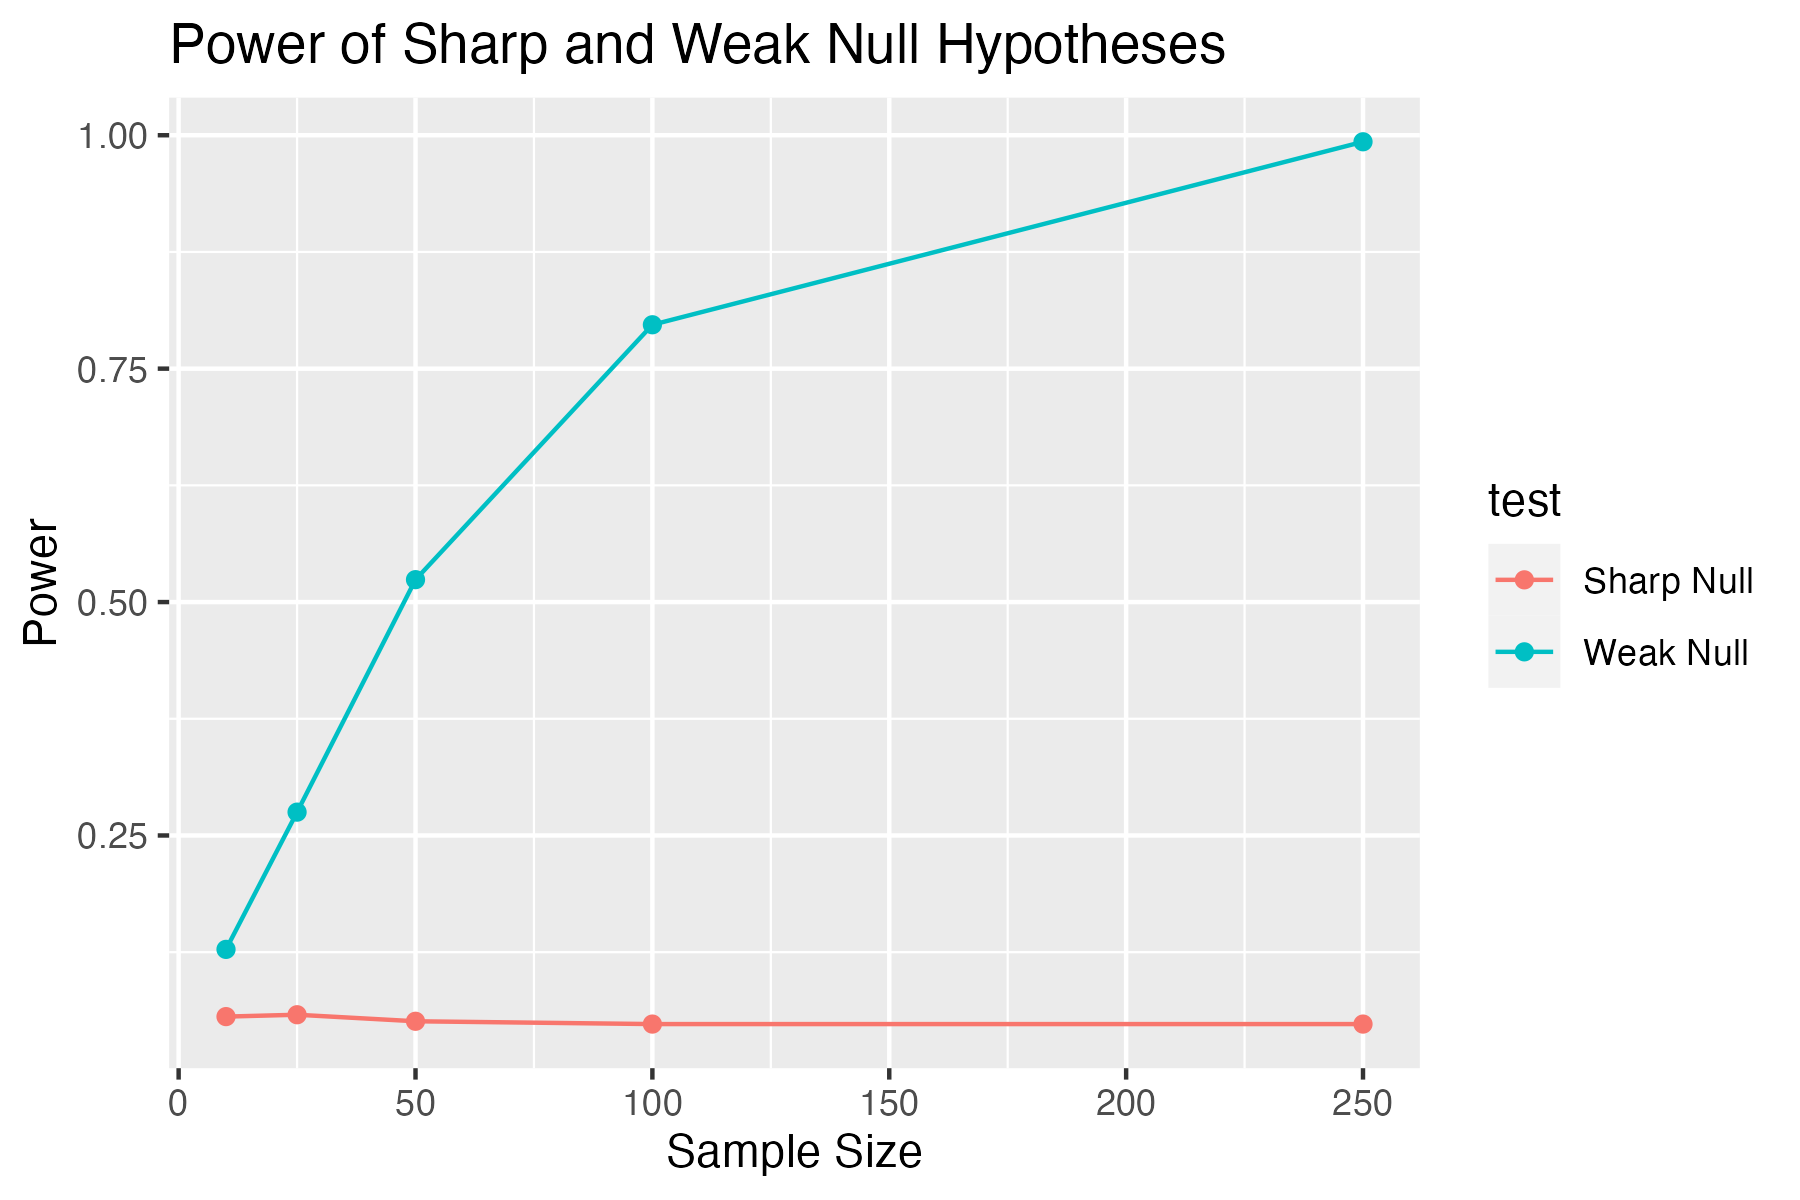
\includegraphics[width=6in,height=\textheight]{power_curve.png}

The visualization rendered shows how our power to test the weak null
rapidly increases with our sample size, while the power to test the
sharp null remains at basically zero. While this is not damning evidence
against the sharp-null hypothesis per-se, it does represent a very real
practical challenge in using the sharp-null hypothesis. While vigorous
debates about whether the sharp null or weak null hypothesis is more
appropriate may ensue, certainly most practically minded collaborators
will appreciate that at any sample size we will have more power to test
the weak null and if that suffices to answer key study questions, we
have good reason to argue for testing a weak null as a satisfactory
study endpoint.

\newpage

\hypertarget{question-7}{%
\subsection{Question 7}\label{question-7}}

Consider a completely randomized experiment (CRE) having enrolled
\(i = 1, \ldots, n\) study units, \(m\) of which receive the treatment
condition. Let \(A_i\) be the indicator of the \(i^{th}\) unit having
received the treatment, and, further, define
\(Y^1 = \frac{1}{m} \sum_{i=1}^n A_i Y_i\) be the average outcome of the
treated units, and similarly define \(Y^0\). You have been tasked with
estimating the average treatment effect (ATE), for which it suffices to
solve the following least squares program:

\[
\min_{\alpha,\beta} \frac{1}{2n} \sum_{i=1}^n (Y_i - \alpha - \beta A_i)^2
\]

\begin{enumerate}
\def\labelenumi{\alph{enumi})}
\item
  Solve the linear program in \((\alpha, \beta)\) to obtain solutions
  for each of the two parameters, denoting these
  \((\hat{\alpha}, \hat{\beta})\).
\item
  Is \(\hat{\beta}\) a valid estimator of the ATE? Explain your answer.
\end{enumerate}

\hypertarget{answers-to-question-7}{%
\subsection{Answers to Question 7}\label{answers-to-question-7}}

\begin{enumerate}
\def\labelenumi{\alph{enumi})}
\tightlist
\item
  The least squares program can be solved by taking the partial
  derivatives of the objective function with respect to \(\alpha\) and
  \(\beta\), and setting them equal to zero. This yields the following
  system of equations:
\end{enumerate}

\[
\begin{aligned}
\pp{\alpha} \frac{1}{2n} \sum_{i=1}^n (Y_i - \alpha - \beta A_i)^2 & = 0 \\
\pp{\beta} \frac{1}{2n} \sum_{i=1}^n (Y_i - \alpha - \beta A_i)^2 & = 0 .
\end{aligned}
\]

Solving these equations yields the following solutions:

\[
\begin{aligned}
\hat{\alpha} & = \bar{Y} - \hat{\beta} \bar{A} \\
\hat{\beta} & = \frac{\sum A_i Y_i - \hat \alpha \sum A_i }{\sum A_i^2}.
\end{aligned}
\]

Now note that \(A_i^2 = A_i\) since \(A_i\) is binary, and specifically
\(\sum A_i = m\), so we have that
\(\hat \beta = \frac{m Y^1}{m} - \hat \alpha = Y^1 - \hat \alpha\).

\begin{enumerate}
\def\labelenumi{\alph{enumi})}
\setcounter{enumi}{1}
\tightlist
\item
  As long as we have that \(m > 0\), then yes, \(\hat \beta\) is a valid
  estimator for the ATE. Since we are in the completely randomized
  experimental setting, we have that the necessary assumptions for
  \(\hat \beta\) to be a valid estimator hold: namely, randomization,
  consistency, and positivity.
\end{enumerate}

Since the treatment is binary, \(\hat \beta\) captures the average
difference between the treated and untreated group, and since we have
randomized the treatment, we know that there is no potential for
confounding.

Threats to the validity of \(\hat \beta\) include if there were
treatment non-compliance, interference, or spillover effects.

\newpage

\hypertarget{code-appendix}{%
\subsection{Code Appendix}\label{code-appendix}}

\hypertarget{code-for-question-6}{%
\subsubsection{Code for Question 6}\label{code-for-question-6}}

\begin{Shaded}
\begin{Highlighting}[]
\FunctionTok{set.seed}\NormalTok{(}\DecValTok{1234}\NormalTok{)}
\FunctionTok{library}\NormalTok{(magrittr)}
\FunctionTok{library}\NormalTok{(dplyr)}
\FunctionTok{library}\NormalTok{(ggplot2)}

\NormalTok{n1 }\OtherTok{\textless{}{-}} \FunctionTok{c}\NormalTok{(}\DecValTok{10}\NormalTok{, }\DecValTok{25}\NormalTok{, }\DecValTok{50}\NormalTok{, }\DecValTok{100}\NormalTok{, }\DecValTok{250}\NormalTok{)}
\NormalTok{n0 }\OtherTok{\textless{}{-}}\NormalTok{ n1}
\NormalTok{n\_sim }\OtherTok{\textless{}{-}}\NormalTok{ 1000L}
\NormalTok{B }\OtherTok{\textless{}{-}}\NormalTok{ 10000L}
\NormalTok{alpha }\OtherTok{\textless{}{-}} \FloatTok{0.05}

\CommentTok{\# Simulate data and test the sharp and weak nulls}
\NormalTok{simulate\_and\_test\_null\_hypotheses }\OtherTok{\textless{}{-}} \ControlFlowTok{function}\NormalTok{(B, n1, n0) \{}

\NormalTok{  sharp\_p\_values }\OtherTok{\textless{}{-}} \FunctionTok{numeric}\NormalTok{(}\AttributeTok{length=}\NormalTok{B) }
\NormalTok{  weak\_p\_values }\OtherTok{\textless{}{-}} \FunctionTok{numeric}\NormalTok{(}\AttributeTok{length=}\NormalTok{B) }

  \ControlFlowTok{for}\NormalTok{ (i }\ControlFlowTok{in} \DecValTok{1}\SpecialCharTok{:}\NormalTok{B) \{}
    \CommentTok{\# simulate potential outcomes}
\NormalTok{    Y1 }\OtherTok{\textless{}{-}} \FunctionTok{rnorm}\NormalTok{(n1}\SpecialCharTok{+}\NormalTok{n0, }\AttributeTok{mean =} \DecValTok{1}\SpecialCharTok{/}\DecValTok{10}\NormalTok{, }\AttributeTok{sd =} \DecValTok{1}\SpecialCharTok{/}\DecValTok{4}\NormalTok{)}
\NormalTok{    Y0 }\OtherTok{\textless{}{-}} \FunctionTok{rnorm}\NormalTok{(n1}\SpecialCharTok{+}\NormalTok{n0, }\AttributeTok{mean =} \DecValTok{0}\NormalTok{, }\AttributeTok{sd =} \DecValTok{1}\SpecialCharTok{/}\DecValTok{4}\NormalTok{)}
\NormalTok{    A }\OtherTok{\textless{}{-}} \FunctionTok{rbinom}\NormalTok{(n1}\SpecialCharTok{+}\NormalTok{n0, }\AttributeTok{size =} \DecValTok{1}\NormalTok{, }\AttributeTok{prob =} \FloatTok{0.5}\NormalTok{)}

\NormalTok{    test\_stat }\OtherTok{\textless{}{-}}\NormalTok{ (}\DecValTok{1}\SpecialCharTok{/}\FunctionTok{sum}\NormalTok{(A)) }\SpecialCharTok{*} \FunctionTok{sum}\NormalTok{(A }\SpecialCharTok{*}\NormalTok{ Y1) }\SpecialCharTok{{-}} 
\NormalTok{      (}\DecValTok{1}\SpecialCharTok{/}\FunctionTok{sum}\NormalTok{(}\DecValTok{1} \SpecialCharTok{{-}}\NormalTok{ A)) }\SpecialCharTok{*} \FunctionTok{sum}\NormalTok{((}\DecValTok{1} \SpecialCharTok{{-}}\NormalTok{ A) }\SpecialCharTok{*}\NormalTok{ Y0) }

    \CommentTok{\# simulate the null distribution}
\NormalTok{    null\_dist }\OtherTok{\textless{}{-}} \FunctionTok{replicate}\NormalTok{(B, \{}
\NormalTok{      Y1\_perm }\OtherTok{\textless{}{-}}\NormalTok{ Y1}
\NormalTok{      Y0\_perm }\OtherTok{\textless{}{-}}\NormalTok{ Y0}
\NormalTok{      A\_perm }\OtherTok{\textless{}{-}} \FunctionTok{sample}\NormalTok{(A)}
      \CommentTok{\# test statistic calculated on the null distribution:}
\NormalTok{      (}\DecValTok{1}\SpecialCharTok{/}\FunctionTok{sum}\NormalTok{(A\_perm)) }\SpecialCharTok{*} \FunctionTok{sum}\NormalTok{(A\_perm }\SpecialCharTok{*}\NormalTok{ Y1\_perm) }\SpecialCharTok{{-}} 
\NormalTok{        (}\DecValTok{1}\SpecialCharTok{/}\FunctionTok{sum}\NormalTok{(}\DecValTok{1} \SpecialCharTok{{-}}\NormalTok{ A\_perm)) }\SpecialCharTok{*} \FunctionTok{sum}\NormalTok{((}\DecValTok{1} \SpecialCharTok{{-}}\NormalTok{ A\_perm) }\SpecialCharTok{*}\NormalTok{ Y0\_perm)}
\NormalTok{    \})}

    \CommentTok{\# calculate and store p{-}values}
\NormalTok{    sharp\_p\_values[i] }\OtherTok{\textless{}{-}} \FunctionTok{mean}\NormalTok{(null\_dist }\SpecialCharTok{\textgreater{}}\NormalTok{ test\_stat)}
\NormalTok{    weak\_p\_values[i] }\OtherTok{\textless{}{-}} \FunctionTok{tryCatch}\NormalTok{(\{}
      \FunctionTok{t.test}\NormalTok{(Y1[A }\SpecialCharTok{==} \DecValTok{1}\NormalTok{], Y0[A }\SpecialCharTok{==} \DecValTok{0}\NormalTok{])}\SpecialCharTok{$}\NormalTok{p.value \},}
      \AttributeTok{error =} \ControlFlowTok{function}\NormalTok{(e) \{ }\ConstantTok{NA}\NormalTok{ \}) }\CommentTok{\# handles when A is all 0 or all 1 }
\NormalTok{  \}}

  \FunctionTok{return}\NormalTok{(}\FunctionTok{data.frame}\NormalTok{(}
    \AttributeTok{sharp\_p\_values\_w\_power =} \FunctionTok{mean}\NormalTok{(sharp\_p\_values }\SpecialCharTok{\textless{}}\NormalTok{ alpha), }
    \AttributeTok{weak\_p\_values\_w\_power =} \FunctionTok{mean}\NormalTok{(weak\_p\_values }\SpecialCharTok{\textless{}}\NormalTok{ alpha)))}
\NormalTok{\}}

\CommentTok{\# Run simulations with different sample sizes}
\NormalTok{results }\OtherTok{\textless{}{-}} \FunctionTok{list}\NormalTok{()}
\ControlFlowTok{for}\NormalTok{ (i }\ControlFlowTok{in} \DecValTok{1}\SpecialCharTok{:}\FunctionTok{length}\NormalTok{(n1)) \{}
\NormalTok{  results[[}\FunctionTok{length}\NormalTok{(results)}\SpecialCharTok{+}\DecValTok{1}\NormalTok{]] }\OtherTok{\textless{}{-}} 
    \FunctionTok{bind\_cols}\NormalTok{(}\AttributeTok{n =}\NormalTok{ n1[i], }\FunctionTok{simulate\_and\_test\_null\_hypotheses}\NormalTok{(B, n1[i], n0[i]))}
\NormalTok{\}}

\CommentTok{\# Construct data frame of results}
\NormalTok{results\_df }\OtherTok{\textless{}{-}} \FunctionTok{bind\_rows}\NormalTok{(results)}

\CommentTok{\# Visualize the power curve}
\NormalTok{results\_df }\SpecialCharTok{|\textgreater{}} 
\NormalTok{  tidyr}\SpecialCharTok{::}\FunctionTok{pivot\_longer}\NormalTok{(}
    \AttributeTok{cols =} \FunctionTok{c}\NormalTok{(sharp\_p\_values\_w\_power, weak\_p\_values\_w\_power),}
    \AttributeTok{names\_to =} \StringTok{"test"}\NormalTok{,}
    \AttributeTok{values\_to =} \StringTok{"power"}
\NormalTok{  ) }\SpecialCharTok{|\textgreater{}} 
  \FunctionTok{mutate}\NormalTok{(}\AttributeTok{test =} \FunctionTok{ifelse}\NormalTok{(}
\NormalTok{    test }\SpecialCharTok{==} \StringTok{"sharp\_p\_values\_w\_power"}\NormalTok{, }\StringTok{"Sharp Null"}\NormalTok{, }\StringTok{"Weak Null"}\NormalTok{)) }\SpecialCharTok{|\textgreater{}}
  \FunctionTok{ggplot}\NormalTok{(}\FunctionTok{aes}\NormalTok{(}\AttributeTok{x =}\NormalTok{ n, }\AttributeTok{y =}\NormalTok{ power, }\AttributeTok{color =}\NormalTok{ test, }\AttributeTok{group =}\NormalTok{ test)) }\SpecialCharTok{+} 
  \FunctionTok{geom\_line}\NormalTok{() }\SpecialCharTok{+} 
  \FunctionTok{geom\_point}\NormalTok{() }\SpecialCharTok{+} 
  \FunctionTok{xlab}\NormalTok{(}\StringTok{"Sample Size"}\NormalTok{) }\SpecialCharTok{+} 
  \FunctionTok{ylab}\NormalTok{(}\StringTok{"Power"}\NormalTok{) }\SpecialCharTok{+} 
  \FunctionTok{ggtitle}\NormalTok{(}\StringTok{"Power of Sharp and Weak Null Hypotheses"}\NormalTok{)}
\end{Highlighting}
\end{Shaded}




\end{document}
